\chapter{多用途边界处理}

% Sec 3.1
\section{动机}
流固耦合对于复杂的视觉现象仿真有很重要的作用,流体和固体之间的相互作用对两者的运动皆有影响,从而成为一个时间上的迭代过程。这种相互作用在数值上的计算是非常复杂的,并且,在有薄壳或细棒的场景中,流固耦合的计算是更加艰巨的。我们这里定义的薄壳或细棒是在某一个或某两个维度上非常狭窄的物体,以至于在这些维度上,物体的大小是远小于网格的尺度的。由于薄壳或细棒的这种特性,它们的特征在网格中很难被捕捉到,以至于经常

% Recent approaches have demonstrated efficient and realistic simulations of shells~\cite{DiscreteShells,Bridson:2003} or rods \cite{DiscreteRods} in \emph{viscous fluids}~\cite{Fei-2018,Takahashi:2019,Fei-2019}, for which momentum transfer can be carried out both stably and efficiently using reduced models, as well as in \emph{non-turbulent flows} through cut cells~\cite{Azevedo-2016}. Progress in kinetic approaches have even led to stable and much more efficient treatment of coupling in \emph{turbulent flows} via a diffuse-interface immersed boundary method~\cite{Li-2018,Li-2020};
% alas, non-volumetric structures such as thin obstacles are not supported, greatly limiting the variety of simulation scenarios in practice. \smallskip

% In this paper, we introduce an efficient and versatile approach for solving two-way fluid-solid coupling with complex solid shapes (involving both thick or thin structures) within the framework of kinetic fluid simulation. %~\cite{Li-2018,Li-2020}.
% Our algorithm improves on the robustness and visual plausibility of the bounce-back scheme~\cite{Ladd-1994} through the addition of a new velocity correction, resolving the typical shortcomings of the sharp-interface immersed boundary method~\cite{mittal-2008} used in kinetic fluid simulation.
% %In addition, approximations are also proposed for cut-cell-based geometric computations so that the whole solver can run very efficiently.
% The resulting hybrid coupling approach is local and conservative, preserves the highly parallelizable nature of kinetic fluid simulation containing all types of solids (arbitrary-shaped volumes, shells, and rods), and further improves boundary treatment of dynamic solids without having recourse to time rescaling~\cite{Li-2020}.
% In addition, due to new geometric approximations and implementation-level GPU optimizations, our two-way coupling runs even faster than the state-of-the-art kinetic fluid simulation method of Chen \emph{et al.}~\shortcite{Chen-2021} --- typically 4 times faster at a normal grid resolution using recent GPU architectures.

% \subsection{Rationale}\label{sec:movitations}
% Since LBM uses a regular grid to discretize space, fluid-solid interactions are not trivial to enforce correctly: given a solid object immersed in a fluid, its boundary usually does \emph{not} align with the fluid grid, resulting in the existence of ``\emph{cut-cells}'', i.e., \textit{grid cells containing a solid boundary surface}, thus only partially filled with fluid --- see the green cell in Fig.~\ref{fig:cutcell_and_interpolation} (left) for a 2D example. A kinetic solver must handle these cut-cells differently in order for coupling and boundary conditions to be accounted for. While no existing fluid-solid boundary treatment can boast about being efficient, accurate, and stable enough to properly handle coupling, each family of coupling methods has its own advantages --- and limitations.
% The diffuse-interface immersed boundary (DI-IB) method, for instance, bypasses the need to track fresh/non-fresh cells that many bounce-back-based techniques necessitate, and thus maintains its high parallelism, but it typically induces stiff penalty forces that require time rescaling to ensure stability, and fails on thin structures as force spreading is done on both sides of the thin solid.
% On the other hand, bounce-back schemes do prevent flow penetration at the mesoscopic level, but their accuracy is limited due to their lattice-based nature, yielding non-smooth spurious velocity distributions around solid and inducing coupling instability in turbulent flow simulations.

% Our hybrid approach stems from the fact that these two families of coupling strategies are, in essence, \textit{complementary}.
% While they are inaccurate for handling thin solid structures, bounce-back schemes directly enforce non-penetration by bouncing distribution functions off solid boundaries, which, in effect, partially accounts for the penalty forces that the IB method would have generated instead. Thus, we can add ancillary penalty forces \emph{after} the bounce-back scheme has been applied in order to further correct the velocity field near the solid boundary. Note that these ancillary forces will be \emph{far weaker} than in usual IB methods as the bounce-back scheme has already applied an impulse to the fluid, thus not necessitating time rescaling (i.e., smaller time steps). \emph{If we can modify the bounce-back scheme to support coupling with thin solids as well, a hybrid approach combining bounce-back and velocity correction would provide the desired robustness, efficiency, and accuracy needed to handle fluid-solid coupling in an LBM solver, without affecting its degree of parallelism.}
% %However, in order to support dynamic coupling with thin moving solid, we need to modify the traditional bounce-back scheme in an immersed way, together with a cut-cell-based one-sided interpolation so that proper velocity corrections can be achieved by penalty forces near solid boundaries while non-penetration property can still be retained. These two steps altogether result in a momentum change near solid boundaries; thus, a momentum-exchange-based method can be applied to obtain the force and torque on the solid to drive its motion.


% Our hybrid coupling approach implements this idea through three distinct computational stages added to a kinetic solver to handle dynamic fluid-solid interaction:
% \begin{itemize}[leftmargin=4mm,itemsep=0.5ex,labelsep=0.6ex,topsep=0.5ex]

% \item \emph{Double-sided bounce-back (DSBB)}: we introduce in Sec.~\ref{sec:DBB} a variant of the original bounce-back scheme where the usual LBM streaming process is altered for nodes of cut-cells on \emph{both} sides of the solid boundaries to prevent flow penetration and enforce a sided bounce against solid boundaries at the mesoscopic level.

% \item \emph{Velocity correction in cut-cells}: in Sec.~\ref{sec:VelocityCorrection}, we counteract the boundary artifacts that a bounce-back scheme can create through an ancillary velocity correction for cut-cell nodes derived from a one-sided interpolation using simpler geometric approximations to improve boundary subgrid treatment, thus drastically suppressing overshoots and increasing simulation stability.

% \item \emph{Momentum transfer onto solids}: finally, we leverage a combination of momentum exchanges traditionally used at the mesoscopic level in bounce-back schemes and penalty forces during velocity correction to transfer to the solid all the forces exerted by the fluid present in cut-cells in order to drive solid motion.

% \end{itemize}

% Upon completion of our algorithm description, we will present tests and evaluations of our new hybrid boundary treatment method to validate its physical validity and improved accuracy to the typical coupling methods in the literature for LBM.

% %The penetration can be avoided by using bounce-back scheme on top of the diffused immersed boundary method~\cite{Chun-2007} to prevent streaming distribution functions across solid surfaces, which can be applied to both thick solids and thin shells, but still inapplicable for thin rods, and spurious velocities around solids may still occur.
% %Motivated from the existing approaches discussed above, if the penalty forces around the solid boundaries can be more properly computed, together with a bounce-back scheme, it seems possible to develop a more general and more accurate and stable fluid-solid coupling method for the kinetic fluid simulation framework to handle a large variety of solid geometries, which forms the main focus of this paper

% \begin{figure}[t] %\vspace*{0mm}
% 	\centering 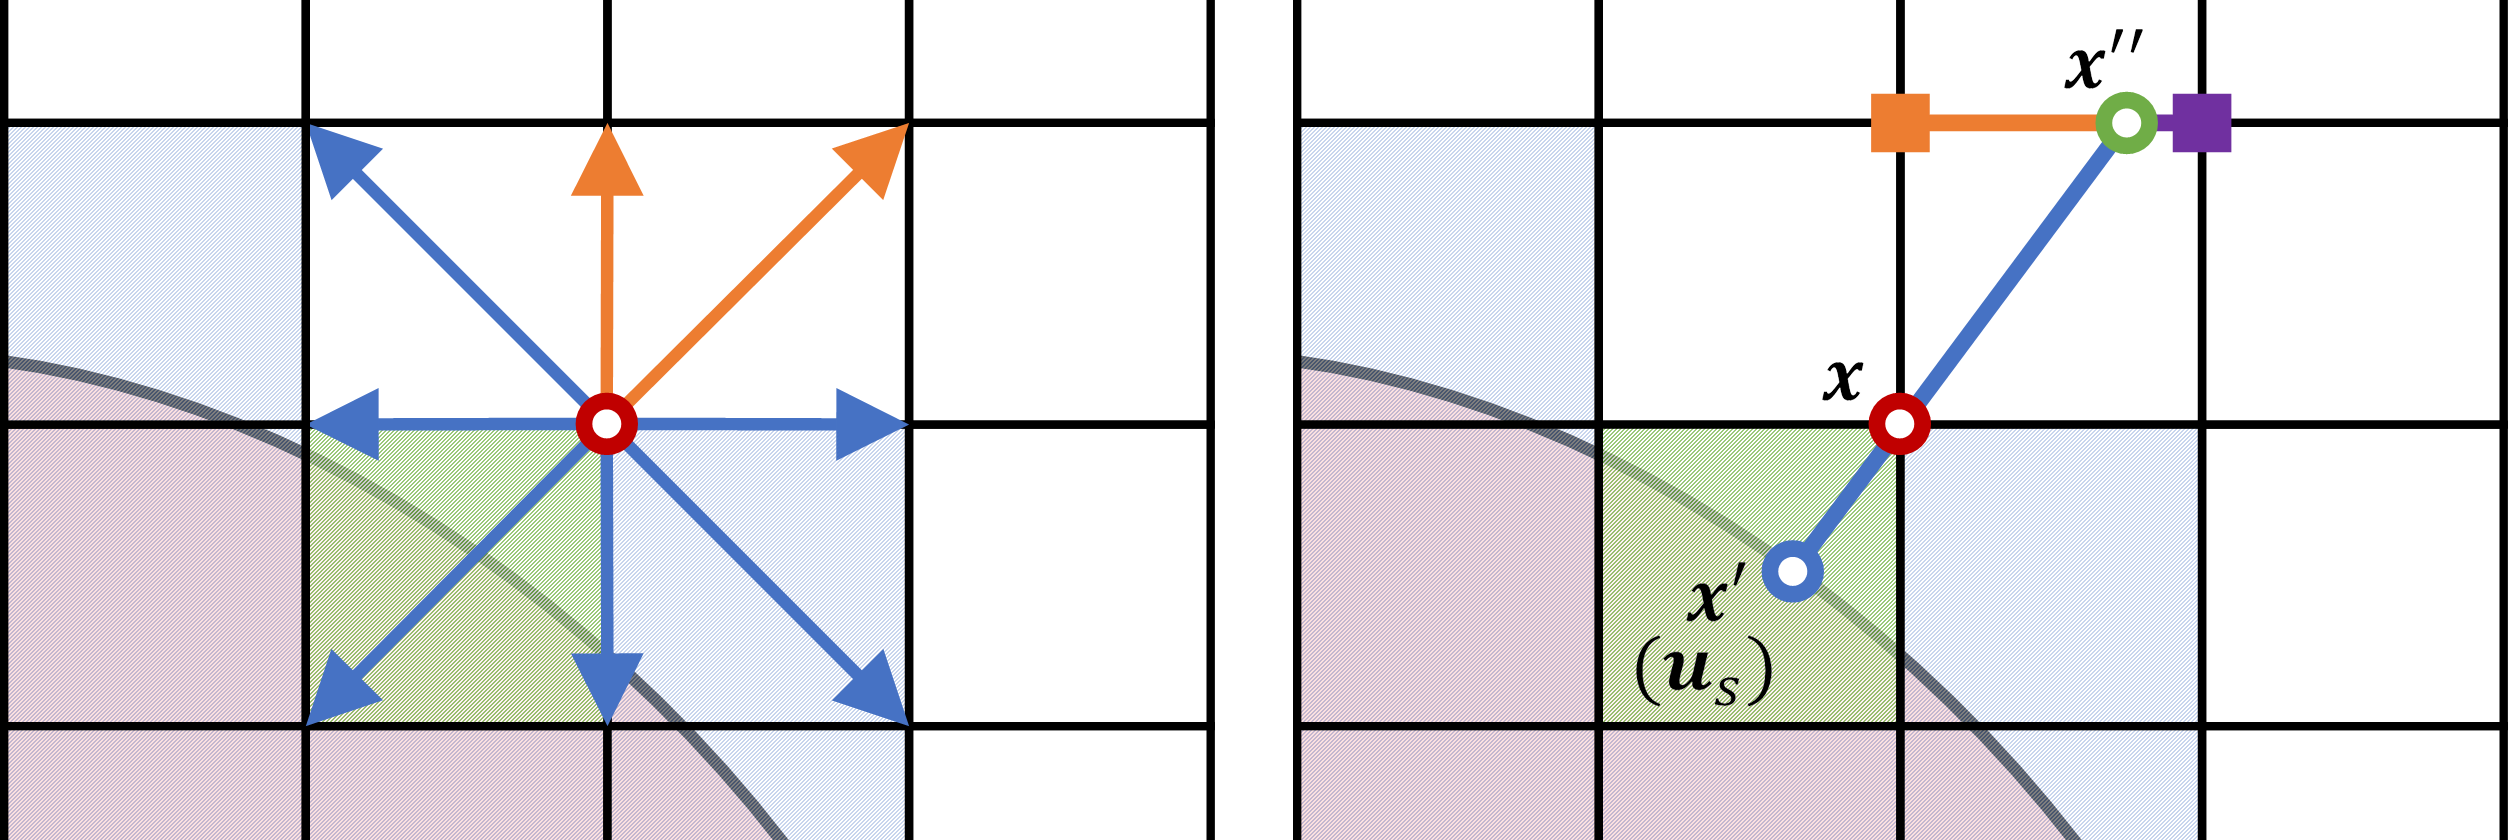
\includegraphics[width=0.96\columnwidth]{images/cutcell_and_interpolation} \vspace*{-3mm}
% 	\caption{\textbf{Interpolation of velocity on cut-cell nodes.} Left: cut-cell (marked in green) intersecting a solid boundary; Right: the velocity on a cut-cell node $\bm{x}$ inside the fluid region (red circle) needs to be interpolated using the velocities of its projected point $\bm{x}{'}$ onto the solid boundary (blue circle) and the intersected point between the ray from the projected point to the cut-cell node and the interpolated fluid point $\bm{x}{''}$ (green circle), where the velocity can be reliably evaluated through simple linear interpolation.		\vspace*{-3mm}}
% 	\label{fig:cutcell_and_interpolation}
% \end{figure}